\section*{Question 7}
\fakesection{7}

This problem compares the Good-Thomas FFT algorithm with the other algorithms implemented in Question 6. The Good-Thomas algorithm is visualised in Figure \ref{fig:q7_viz_good_thomas}.

\begin{figure}[ht]
    \centering
    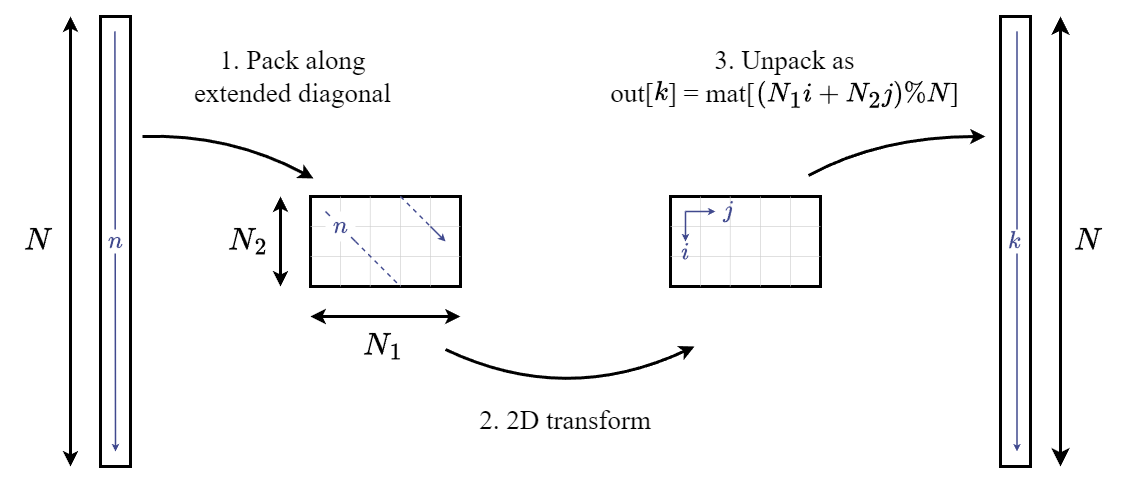
\includegraphics[width=0.85\textwidth]{images/q7_viz_good_thomas.png}
    \caption{Visualisation of the Good-Thomas algorithm}
    \label{fig:q7_viz_good_thomas}
\end{figure}

In words, where $N_1N_2=N$, the algorithm:
\begin{enumerate}
    \item Constructs an $N_1\times N_2$ matrix along the extended diagonal; time complexity in $\Theta(N)$.
    \item Performs DFT on each column and row; in $\Theta(N_1N_2^2 + N_2N_1^2)$.
    \item Constructs the output signal using the following indexing, in $\Theta(N)$:
    \begin{align*}
        \text{out}[(N_1 i + N_2 j) \text{ mod } N] = \text{mat}[i,j]
    \end{align*}
    where $i$ and $j$ are matrix row and column indices, respectively.
\end{enumerate}
The construction means twiddle factors are not required. The overall time complexity is in:
\begin{align}
    \Theta(N_1N_2^2 + N_2N_1^2)
\end{align}
While the asymptotic time complexity is equal to that of the Cooley-Tukey algorithm, the fact that twiddle factors are not needed means the Good-Thomas algorithm is faster in practice.

Figure \ref{fig:q7_good_thomas} shows the transformed result produced by the Good-Thomas algorithm.

\begin{figure}[ht]
    \centering
    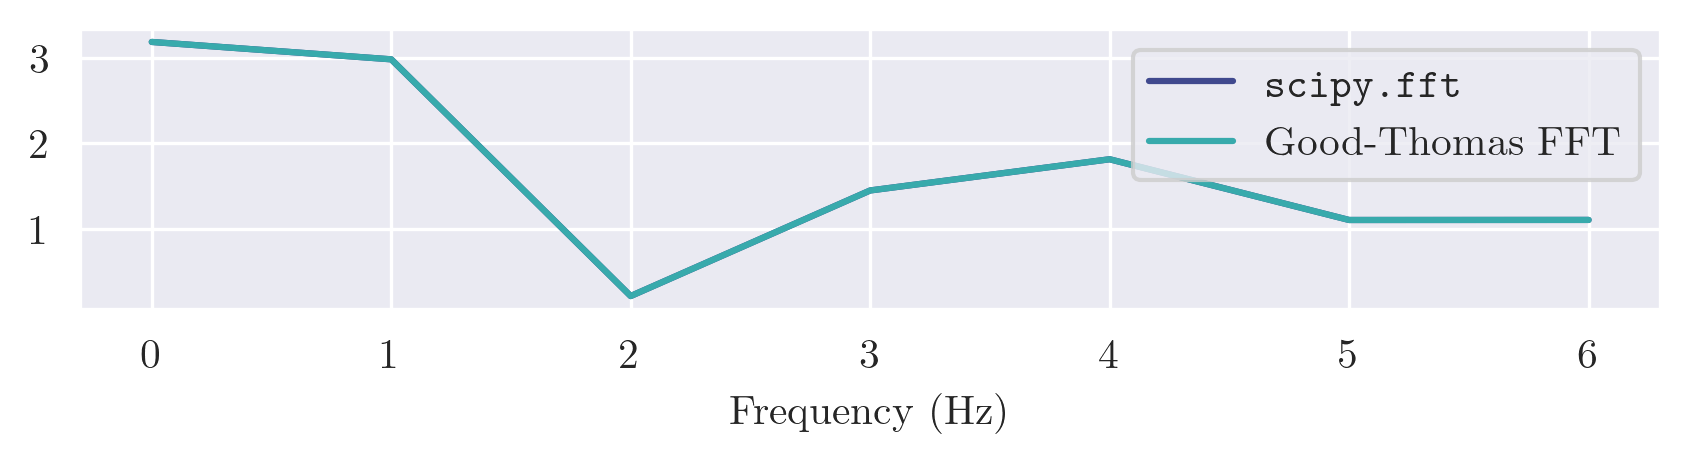
\includegraphics[width=0.8\textwidth]{images/q7_transform.png}
    \caption{Fourier transform by Good-Thomas algorithm}
    \label{fig:q7_good_thomas}
\end{figure}

Table \ref{tab:q7_timings} compares the average timing of the algorithm compared to those from Question 6.

\newpage

\begin{table}[ht]
    \small \centering \restretch{1.2}
    \caption{Average runtime (ms) on 15-point sequence over 10,000 trials}
    \begin{tabularx}{0.7\textwidth}{r R r r}
        \toprule
        \textbf{\texttt{scipy.fft}} & \textbf{DFT} & \textbf{Cooley-Tukey FFT} & \textbf{Good-Thomas FFT} \\
        \midrule
        0.007 & 0.372 & 0.246 & 0.224 \\
        \bottomrule
    \end{tabularx}
    \label{tab:q7_timings}
\end{table}

The Good-Thomas algorithm achieves around 10\% speedup over the Cooley-Tukey algorithm. Again, this is for a short signal; the difference should grow proportionally to signal length (since the number of twiddle factors is proportional to length), which is why the Good-Thomas algorithm is generally preferred over the Cooley-Tukey algorithm.
